\subsection{Can Lighting Requirements Be Met Through the Proposed System?} \label{section:question3}

%New Paragraph
For lighting requirements, as previously discussion in Section \ref{section:draft-floor-plan} there are Australian standards that impact the quantity and types of luminaires. Table \ref{table:LightingRequirements} outlines the lux requirements expressed in AS/NZS 1680.2.2 explaining that the target for a standard office should be between 200\,lux and 300\,lux unless technical work is required (a minimum of 320 is required in this case) \cite{StandardsAustralia2006_2}.
\newline

%New Paragraph
To begin the analysis, the project test model standard office was modelled in the lighting simulation software package Dialux. As discussed in Section \ref{section:project-model} the floor plan is based off of QUT Garden's Point Campus P Block level 6. The reason this was chosen is that it is a real world application of a commercial office floor that access to the schematics and design plans was made available. This was the most accurate method for producing a model that could be applied to industry. 

\subsubsection{Office Room Lighting Model}   

%New Paragraph
The large floor plan shown in Section \ref{section:draft-floor-plan} was loaded into Dialux and an office separated out for modelling. The room was approximation shows that offices on this are 22\,\si{m^2} and this lighting simulation displays this. The fittings modelled were luminaires with the same specifications outlined in the QUT design documents. Specifically, this is the Futcha LED 27.5\,W fitting from Pierlite \cite{website:Pierlite1}. The DWG file additionally outlined some architectural objects including a table which was included in the modelling. 
\newline

%New Paragraph
Utilising Table \ref{table:QUT-lvl6-office-assumptions} below, the assumptions were input into Dialux to complete accurate modelling.
\newline 

\begin{table}[htb]
	\centering
	\renewcommand{\arraystretch}{1}
	\begin{tabular}{|l|l|}
		\hline
		\textbf{Assumption} & \textbf{Value} \\ \hline
		Roof Height         & 2.7m           \\ \hline
		Workplane           & 0.75m          \\ \hline
		Boundaries          & 0.1m           \\ \hline
		Ceiling Reflectance & 70\%           \\ \hline
		Wall Reflectance    & 50\%           \\ \hline
		Floor Reflectance   & 20\%           \\ \hline
	\end{tabular}
	\caption{QUT: P Block Level 7 Office Lighting Simulation Assumptions}
	\label{table:QUT-lvl6-office-assumptions}
\end{table} 

%New Paragraph
The calculation completed in Figure \ref{fig:dialux-office-workplane-summary} was to ensure that the inputs received from the schematics were correctly understood. Appendix \ref{appendix:QUT-Lvl6-office-rev3} shows the complete Dialux output however the important aspects are the lux values of the workplace shown in Figure \ref{fig:dialux-office-workplane-summary} and the 3D render shown in Figure \ref{fig:dialux-office-3D}.  

\begin{figure}[H]
	\hfill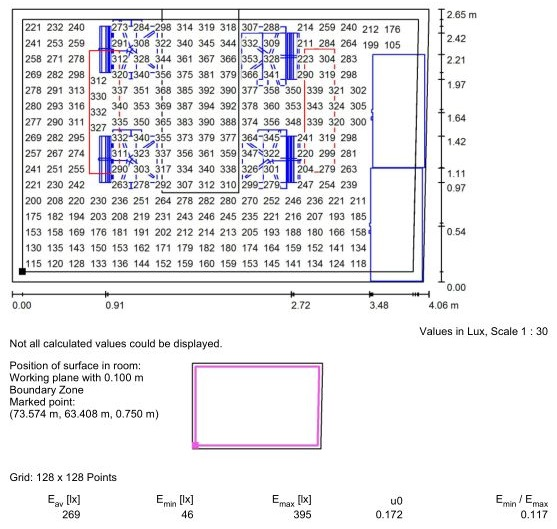
\includegraphics[width = 120mm]{images/project-model/dialux-office-workplane-summary}\hspace*{\fill}
	\caption{QUT: P Block Level 7 Office Lux Analysis} 
	\label{fig:dialux-office-workplane-summary}
\end{figure}

\begin{figure}[H]
	\hfill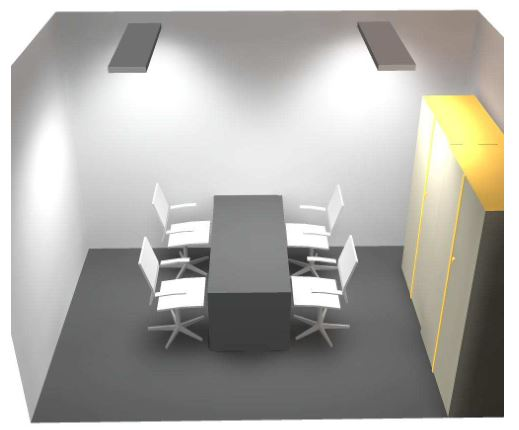
\includegraphics[width = 130mm]{images/project-model/dialux-office-3D}\hspace*{\fill}
	\caption{QUT: P Block Level 7 Office 3D Render} 
	\label{fig:dialux-office-3D}
\end{figure}

\subsubsection{Lighting Model Discussion}
~\\
%New Paragraph
Comparing Figure \ref{fig:dialux-office-3D} to the lighting standards requirements in the below Table \ref{table:LightingRequirements2}, it can be seen that the room is above standard with the average of 269\,lux provided that it's a general office not requiring technical work or visually difficult applications. Table \ref{table:QUTlvl7-count} has the total luminaires count and therefore the total demand for the office level, this will be scaled for the size of a project building.    

\begin{table}[H]
	\centering
	\renewcommand{\arraystretch}{1}
	\begin{tabular}{|l|c|}
		\hline
		\textbf{Area or Application} 	& \textbf{Lux Requirement} \\ \hline
		Rarely Visited 					& 40 \\ \hline
		Storage Rooms or Change Room 	& 80 \\ \hline
		Machine Work or Waiting Room 	& 160 \\ \hline
		Food Preparation Room 			& 240 \\ \hline
		Technical Office Room 			& 320 \\ \hline
		Visually Difficult Work 		& 500 \\ \hline
	\end{tabular}
	\caption{Lighting Requirements as per AS/NZS Standards \cite{StandardsAustralia2006_2}}
	\label{table:LightingRequirements2}
\end{table}  


\subsubsection{Equipment Improvements}

%New Paragraph
~\\
As discussed in Section \ref{litreview:dc-devices} of the Literature review, with the growth of DC distribution more devices are becoming available. For the project model, LED devices will be used for higher efficiency and of course the ballasts will be required to receive 48\,V\,DC and output specific LED fitting requirements.  

